\begin{defn}
    The \textit{Dirichlet function }on $[0,1]$ is 
    \begin{equation}
        \label{Equ:Diri_Func}
        D(x)=\left\{
            \begin{array}{rl}
                1&x\in \mathbb{Q},\\
                0&x\notin\mathbb{Q}.
            \end{array}
        \right.
    \end{equation}
\end{defn}
\begin{exc}
    Show \eqref{Equ:Diri_Func} isn't Riemann integrable on $[0,1]$.
\end{exc}
\begin{proof}
    If $\Delta$ is a partition on $[0,1]$,
    \begin{displaymath}
        \Delta:0<x_1<x_2<\ldots<x_n=1,
    \end{displaymath}
    Set $\xi=(\xi_n)$, where $\xi_k\in[x_{k-1},x_k]$ is rational number,
    then $S(\Delta,\xi)=\sum_{k=1}^{n}D(\xi_k)\Delta x_K=1$.
    However, if set $\eta=(\eta_n)$, where $\eta_k\in[x_{k-1},x_k]$
    is irrational number, 
    then $S(\Delta,\eta)=\sum_{k=1}^{n}D(\eta_k)\Delta x_K=0$, 
    which means $\lim_{||\Delta||\rightarrow 0}S(\Delta,\xi)=1$,
    but $\lim_{||\Delta||\rightarrow 0}S(\Delta,\eta)=0$. 
    $D(x)$ is not Riemann integrable on $[0,1]$.
\end{proof}
\begin{rem}
    $D(x)=0$ a.e. on $[0,1]$, so we expact $\int_{0}^{1}D(x)\dif x=0$, 
    but $D(x)$ isn't Riemann integrable. 
    In this chapter, we introduce \textit{Lebesgue integral} to 
    handle this problem.
\end{rem}
\section{Measurable Functions}
\begin{defn}
    \label{Def:Preimage}
    Given a function $f:X\rightarrow Y$, $E\subset Y$, 
    \begin{displaymath}
        f^{-1}(E):=\{x\in X:f(x)\in E\}
    \end{displaymath}
    is the \textit{preimage} of $E$ related to $f$.
\end{defn}
\begin{prop}
    \label{Prop:PreimageProp}
    \begin{enumerate}
        \item $f^{-1}(\cup_{\lambda}E_{\lambda})
        =\cup_{\lambda}f^{-1}(E_{\lambda})$. 
        \item $f^{-1}(\cap_{\lambda}E_{\lambda})
        =\cap_{\lambda}f^{-1}(E_{\lambda})$.
        \item $f^{-1}(E^c)=(f^{-1}(E))^{c}$.
        \item If $\mathcal{N}$ is a $\sigma$-algebra on $Y$, 
        then $\{f^{-1}(E):E\in\mathcal{N}\}$ is a 
        $\sigma$-algebra on $X$.
    \end{enumerate}
\end{prop}
\begin{exc}
    Prove Proposition \ref{Prop:PreimageProp}.
\end{exc}
\begin{proof}
    For the first rule, $\forall x\in f^{-1}(\cup_{\lambda}E_{\lambda})$,
    $f(x)\in\cup_{\lambda}E_{\lambda}$, so $\exists \lambda_x$, s.t.
    $f(x)\in E_{\lambda_x}$, which means $x\in f^{-1}(E_{\lambda_x})$,
    so $x\in \cup_{\lambda}f^{-1}(E_{\lambda})$. On the other hand,
    $\forall y\in\cup_{\lambda}f^{-1}(E_{\lambda})$, 
    $\exists \lambda_y$, s.t. $y\in f^{-1}(E_{\lambda_y})$,
    so $y\in f^{-1}(\cup_{\lambda}E_{\lambda})$. 
    Thus, it's easy to conclude that  
    $f^{-1}(\cup_{\lambda}E_{\lambda})
    =\cup_{\lambda}f^{-1}(E_{\lambda})$.

    The second rule can be proved in the same way as the first one.

    As for the third one, $\forall x\in f^{-1}(E^c)$, so $f(x)\notin E$,
    which means $x\in(f^{-1}(E))^{c}$. On the other hand,
    $\forall y\in(f^{-1}(E))^{c}$, so $y\notin f^{-1}(E)$,
    which means $f(y)\in E^c$, so $y\in f^{-1}(E^c)$.
    Thus, it's easy to conclude that $f^{-1}(E^c)=(f^{-1}(E))^{c}$.

    The fourth rule can be easily proved by the first three rules
    and the Definition \ref{Defn:SigmaAlg}.
\end{proof}
\begin{defn}
    \label{Def:MeasurableFunc}
    If $(X,\M)$, $(Y,\mathcal{N})$ are measurable spaces, 
    $f:X\rightarrow Y$ is called \textit{$(\M,\mathcal{N})$-measurable} 
    if $\forall E\in\mathcal{N}$, $f^{-1}(E)\in\M$.
\end{defn}
\begin{prop}
    \label{Prop:DescribeMeasFunc}
    If $\mathcal{N}=\M(\mathcal{E})$, then $f:X\rightarrow Y$ is 
    measurable iff $\forall E\in\mathcal{E}$, $f^{-1}(E)\in\M$.
\end{prop}
\begin{proof}
    $"\Rightarrow"$: Follows directly by Definition 
    \ref{Def:MeasurableFunc}.
    
    $"\Leftarrow"$: By Proposition \ref{Prop:PreimageProp}, 
    $\mathcal{A}:=\{E\subset Y:f^{-1}(E)\in\M\}$ is a $\sigma$-algebra, 
    and by the condition, this $\sigma$-algebra contains $\mathcal{E}$, 
    so $\mathcal{A}\supset\mathcal{M}(\mathcal{E})=\mathcal{N}$, 
    i.e. $f$ is a measurable function.  
\end{proof}
\begin{coro}
    \label{Cor:ContinuousMeas}
    If $(X,\tau_1)$, $(Y,\tau_2)$ are topological spaces and 
    $f:X\rightarrow Y$ is continuous, then 
    $f$ is $(\mathcal{B}_{X},\mathcal{B}_{Y})$-measurable.
\end{coro}
\begin{exc}
    Prove Corollary \ref{Cor:ContinuousMeas}.
\end{exc}
\begin{proof}
    $f:X\rightarrow Y$ is continuous $\Leftrightarrow$ 
    $\forall U\in\tau_2$, $f^{-1}(U)\in\tau_1$.
    By Definition \ref{Def:MeasurableFunc}, we know
    $f$ is $(\mathcal{B}_{X},\mathcal{B}_{Y})$-measurable.
\end{proof}
\begin{defn}
    \label{Defn:Mmeasurable}
    Given $(X,\M)$ be a measurable space, $f:X\rightarrow\mathbb{R}$ 
    (or $\mathbb{C}$) 
    is called \textit{$\M-$measurable} if $f$ is 
    $(\M,\mathcal{B}_{\mathbb{R}})$ (or $(\M,\mathcal{B}_{\mathbb{C}})$) 
    measurable.
\end{defn}
\begin{defn}
    $f:\mathbb{R}\rightarrow\mathbb{C}$ is \textit{Lebesgue Measurable} 
    if it is $(\mathcal{L},\mathcal{B}_{\mathbb{C}})$-measurable, 
    $f$ is Borel measurable if it is 
    $(\mathcal{B}_{\mathbb{R}},\mathcal{B}_{\mathbb{C}})$-measurable.
\end{defn}
\begin{exc}
    \label{Exc:ComposeOfMeasurable}
    Assume $f,g:\mathbb{R}\rightarrow\mathbb{R}$, 
    If $f$ is Borel measurable and $g$ is Lebesgue measurable, 
    then $f\circ g$ is Lebesgue measurable.
\end{exc}
\begin{proof}
    $\forall E\in\mathcal{B}_{\mathbb{R}}$,by $f$ is Borel measurable,
    so $f^{-1}(E)\in\mathcal{B}_{\mathbb{R}}$, and by 
    $g$ is Lebesgue measurable, $(f\circ g)^{-1}(E)=
    g^{-1}(f^{-1}(E))\in\mathcal{L}$, then $f\circ g$ is Lebesgue measurable.
\end{proof}
\begin{defn}
    \label{Defn:CantorFunc}
    If $\mathcal{C}$ is the \textit{Cantor set} on $[0,1]$
    (see Definition \ref{Defn:CantorSet}), 
    the \textit{Cantor function} $c:[0,1]\rightarrow[0,1]$ 
    is:
    \begin{equation}
        \label{Equ:CantorFunc}
        c(x)=\left\{
            \begin{array}{rl}
                \sm{n}{\infty}\frac{a_n}{2^{n}},&
                x=\sm{n}{\infty}\frac{2a_n}{3^n}\in\mathcal{C}
                ;\\
                \sup_{y\le x,y\in\mathcal{C}}c(y),&x\in[0,1]\setminus
                \mathcal{C}.\\
            \end{array}
        \right.
    \end{equation}
    \begin{figure}[H]
        \centering
        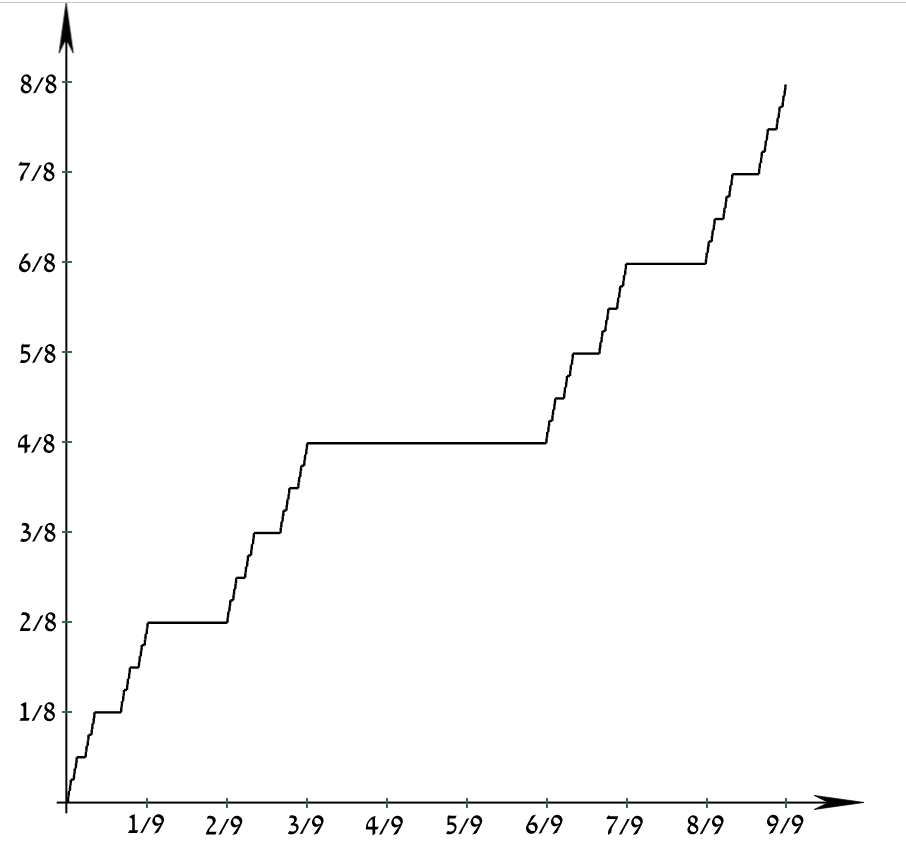
\includegraphics
        [width=\linewidth,height=0.2\textheight]{png/CantorFunc.png}
        \caption{Cantor function, download from Wikipedia.}
    \end{figure}
\end{defn}
\begin{exc}
    Let $f:[0,1]\rightarrow[0,1]$ be the Cantor function, 
    and let $g(x)=f(x)+x$.
    \begin{enumerate}
        \item $g$ is a bijection from $[0,1]$ to $[0,2]$, 
        and $h=g^{-1}$ is continuous from $[0,2]$ to $[0,1]$.
        \item If $C$ is a Cantor set, $m(g(C))=1$.
        \item $g(C)$ contains a Lebesgue nonmeasurable set $A$. 
        Let $B=g^{-1}(A)$, $B$ is Lebesgue measurable but not Borel.
        \item There exist a Lebesgue measurable function $F$ and a 
        continuous function $G$ on $\mathbb{R}$ such that 
        $F\circ G$ is not Lebesgue measurable.
    \end{enumerate}
\end{exc}
\begin{proof}
    (1)$f(x)$ is monotone increasing, and naturally $p(x)=x$
    is a strictly increasing function, and hence $g(x)=f(x)+x$
    x is also strictly increasing and therefore injective. 
    Next, to show surjectivity, note that $g$ is a continuous function, 
    and $g(0)=0$, $g(1)=2$; hence, by the intermediate value theorem, 
    $g$ is surjective. We now have all the necessary components to 
    conclude that $g$ is a bijection, and since $g$ is a
    continuous bijective function, and $[0,1]$ is compact, 
    $g^{-1}$ is continuous from $[0,2]$ to $[0,1]$.

    (2)Firstly, by $g$'s surjectivity, and $C$ being measurable, 
    we see that:
    \begin{displaymath}
        \begin{array}{rl}
            g([0,1]\setminus C)\cup g(C)=g([0,1]\cap C^c)\cup g(C)=[0,2]\\
            \Rightarrow m(g(C))+m(g([0,1]\setminus C))=2.
        \end{array}
    \end{displaymath}
    Next, since $C$ is a closed set $\Rightarrow$ $[0,1]\setminus C$
    is open set. Therefore, since all open subsets of $[0,1]$ may
    be written as a countable union of disjoint open sets, 
    let us write $[0,1]\setminus C=\cup_{1}^{\infty}O_j$, $O_j=(a_j,b_j)$.
    Now, since $f$ is by construction constant on $[0,1]\setminus C$,
    and $m(C)=0\Rightarrow m([0,1]\setminus C)=1\Rightarrow
    m(\cup_{1}^{\infty}O_j)=1$.
    \begin{displaymath}
        \begin{array}{rl}
            m(g([0,1]\setminus C))&=m(g(\cup_{1}^{\infty}O_j))=\sum_{1}^{infty}m(g(O_j))\\
            &=\sum_{1}^{infty}(m(f(b_j)-f(a_j))+m(b_j-a_j))\\
            &=\sum_{1}^{infty}m(O_j)\\
            &=m(\cup_{1}^{\infty}O_j)\\
            &=1
        \end{array}
    \end{displaymath}  
    And hence $m(g(C))=1$.
    
    (3)To show Lebesgue measurability, naturally $B\subset C$,
    and since $C$ is measurable with measure $m(C)=0$, it implies
    $m(B)\leq m(C)=0$, and hence Lebesgue measurable since null 
    sets are measurable. For the sake of contradiction, suppose
    $B=g^{-1}(A)$ is Borel measurable. In part (1), we showed that
    $g^{-1}$ is continuous and bijective; therefore 
    $g(B)=g(g^{-1}(A))=A$. However, by the continuity of $g$,
    if $g^{-1}(A)$ was Borel, so too would $g(g^{-1}(A))=A$,
    hence a contradiction since $A$ is not Lebesgue
    measurable; therefore, $B$ cannot be Borel measurable.

    (4)Let $F=\chi_{B}$;
    \begin{equation}
        F(x)=\left\{
            \begin{array}{rl}
                1, &x\in B, \\
                0, &x\notin B,
            \end{array}
        \right.
    \end{equation}
    And also set $G=g^{-1}$. Naturally $G$ is Lebesgue measurable 
    since it is continuous, we now wish to prove that so too is $F$. 
    This can be seen by noticing $F^{-1}((a,\infty))=\emptyset$ or $B$
    or $\mathbb{R}$, , but all these possibilities are Lebesgue measurable,
    hence $F$ is Lebesgue measurable. We can now look at the following 
    reasoning:
    \begin{displaymath}
        \begin{array}{rl}
            (F\circ G)^{-1}([\frac{1}{2},\infty))&=G^{-1}\circ F^{-1}([\frac{1}{2},\infty))\\
            &=\{x\in[0,2]|\chi_B(g^{-1}(x))\in[\frac{1}{2},\infty)\} \\
            &=\{x\in[0,2]|g^{-1}(x)\in B\} \\
            &=G^{-1}(B)=g(g^{-1}(B))=A,
        \end{array}
    \end{displaymath}
    Now since $A$ is not Lebesgue measurable, 
    $F\circ G$ also will not be Lebesgue measurable.
\end{proof}
\begin{prop}
    \label{Prop:ComplexMeasurableFunc}
    $f:X\rightarrow\mathbb{C}$ is $\M$-measurable iff $\text{Re}f$, 
    $\text{Im}f$ are $\M$-measurable. 
\end{prop}
\begin{proof}
    Choose $\pi_{1}(z):=\text{Re}z$, $\pi_{2}(z):=\text{Im}z$, 
    then $\pi_{1},\pi_{2}$ are both measurable. If $f$ is 
    $\M$-measurable, 
    then $\text{Re}f=\pi_{1}\circ f$, $\text{Im}f=\pi_{2}\circ f$ 
    are both $\M$-measurable.

    If $\text{Im}f$, $\text{Re}f$ are both measurable, i.e. 
    $\pi_1\circ f$, $\pi_{2}\circ f$ are measurable, then for 
    any Borel set $\mathcal{B}\subset\mathbb{R}$, 
    $f^{-1}(\pi_{\alpha}^{-1}(\mathcal{B}))\in\M$ for 
    $\alpha=1,2$. $f$ is measurable 
    follows from $\mathcal{B}_{\mathbb{C}}
    =\mathcal{B}_{\mathbb{R}}\otimes
    \mathcal{B}_{\mathbb{R}}$ and 
    Proposition \ref{Prop:DescribeMeasFunc}.
\end{proof}
\begin{prop}
    \label{Prop:MeasFuncLinear}
    If $f,g:X\rightarrow\mathbb{C}$ are 
    $\M$-measurable, so are $f+g$, $fg$. 
\end{prop}
\begin{proof}
    Define $F:X\rightarrow \mathbb{C}\times\mathbb{C}$, 
    $F(x):=(f(x),g(x))$, 
    $\phi,\psi:\mathbb{C}\times\mathbb{C}\rightarrow\mathbb{C}$ 
    are 
    \begin{displaymath}
        \phi(z,w):=z+w,\quad \psi(z,w):=zw,
    \end{displaymath}
    then $F$ is 
    $(\M,\mathcal{B}_{\mathbb{C}\times\mathbb{C}})$-measurable, 
    $\phi,\psi$ are 
    $(\mathcal{B}_{\mathbb{C}\times\mathbb{C}},
    \mathcal{B}_{\mathbb{C}})$-measurable. So are 
    $f+g=\phi\circ F$, $fg=\psi\circ F$.
\end{proof}
\begin{rem}
    Proposition \ref{Prop:MeasFuncLinear} shows that 
    all the $\M$-measurable functions form an algebra.
\end{rem}
\begin{ntn}
    The \textit{generalized real line} 
    is denoted by:
    \begin{displaymath}
        \bar{\mathbb{R}}:=[-\infty,\infty]
        =\mathbb{R}\cup\{-\infty,\infty\}.
    \end{displaymath}
\end{ntn}
\begin{prop}
    \label{Prop:LimitProperties}
    $\forall j\in\mathbb{N}$, 
    $f_{j}:X\rightarrow\bar{\mathbb{R}}$ are 
    measurable functions, then 
    $g_{1}(x):=\limsup_{j\rightarrow\infty}f_{j}(x)$, 
    $g_{2}(x):=\liminf_{j\rightarrow\infty}f_{j}(x)$ 
    are measurable.
\end{prop}
\begin{exc}
    Prove Proposition \ref{Prop:LimitProperties}.
\end{exc}
\begin{proof}
    Set $m(x)=sup_{j}f_{j}(x)$, $n(x)=inf_{j}f_{j}(x)$.
    By the truth that $f_{j}:X\rightarrow\bar{\mathbb{R}}$ are 
    measurable functions, $m^{-1}((a,\infty])=
    \cup_{1}^{\infty}f_{j}^{-1}((a,\infty])$,  $n^{-1}([\infty,a))=
    \cup_{1}^{\infty}f_{j}^{-1}([\infty,a))$, so $m(x)$, $n(x)$
    are measurable. More generally, if $h_k(x)=sup_{j>k}f_j(x)$
    then $h_k$ is measurable for each $k$, so $g_1(x)=inf_{k}h_k(x)$
    is measurable, and likewise for $g_2(x)$.
\end{proof}
\begin{defn}
    Given $f:X\rightarrow\bar{\mathbb{R}}$, 
    the \textit{positive part }of $f$ is:
    \begin{displaymath}
        f^{+}(x):=\max(f(x),0),
    \end{displaymath}
    and the \textit{negative part }of $f$ 
    is:
    \begin{displaymath}
        f^{-}(x):=\max(-f(x),0).
    \end{displaymath}
\end{defn}
\begin{rem}
    If $f$ is measurable, so are $f^{+}$ and 
    $f^{-}$.
\end{rem}
\begin{defn}
    Given $f:X\rightarrow\mathbb{C}$, the 
    \textit{polar decomposition }of $f$ is 
    $f:=(\sgn f)|f|$ where 
    \begin{displaymath}
        \sgn(z)=\left\{
            \begin{array}{rl}
                \frac{z}{|z|},z\neq 0;
                0,z=0.
            \end{array}
        \right.
    \end{displaymath}
\end{defn}
\begin{rem}
    If $f$ is measurable, so are $\sgn f$ and $|f|$.
\end{rem}
\begin{defn}
    \label{Defn:CharFunc}
    For $E\subset X$, the \textit{characteristic function} of $X$ 
    is given by $\chi_{E}(x)$ with:
    \begin{displaymath}
        \chi_{E}(x):=\left\{
            \begin{array}{rl}
                1,x\in E;\\
                0,x\notin E.\\
            \end{array}
        \right.
    \end{displaymath}
\end{defn}
\begin{defn}
    \label{Defn:SimpleFunc}
    A \textit{simple function }on $X$ is given by 
    $f:X\rightarrow\mathbb{C}$ with 
    $f(x)=\sm{j}{n}z_{j}\chi_{E_{j}}$, where $E_j\in\M$, 
    $z_j\in\mathbb{C}$, satisfies $\forall j\neq k$ $z_{j}\neq z_{k}$, 
    $E_j\cap E_k=\emptyset$.
\end{defn}
\begin{thm}
    \label{Thm:ApproxMeasFuncBySimpleFunc}
    If $f:X\rightarrow[0,\infty]$ is measurable, 
    then there exists simple functions $\{\phi_{n}\}$ such that 
    $0\le\phi_{1}\le\ldots\le\phi_{n}\le\ldots\le f$, 
    $\phi_{n}\rightarrow f$ pointwise, and 
    $\phi_{n}\rightarrow f$ uniformly in any set 
    where $f$ is bounded.
\end{thm}
\begin{exc}
    For $0\le k\le 2^{2n}-1$, mark 
    \begin{displaymath}
    E_{n}^{k}:=f^{-1}((k2^{-n},(k+1)2^{-n}]),\quad 
    F_{n}:=f^{-1}((2^{n},\infty]),
    \end{displaymath}
    then define 
    \begin{displaymath}
        \phi_{n}:=\sum_{k=0}^{2^{2n}-1}k2^{-n}\chi_{E_{n}^{k}}
        +2^{n}\chi_{F_{n}},
    \end{displaymath}
    show $\{\phi_{n}\}$ satisfies the condition of 
    Theorem \ref{Thm:ApproxMeasFuncBySimpleFunc}.
\end{exc}
\begin{proof}
    By the truth that $\chi_{E}(x)\geq 0$, it is easily checked
    that $\phi_{n}\leq\phi_{n+1}$ for all $n$, and 
    $0\leq f-\phi_{n}\leq 2^{-n}$ on the set where 
    $f\leq 2^{-n}$. The result therefore follows.
\end{proof}
\section{Integration}
\section{Convergence}
\section{Tonelli-Fubini Theorem}